\nonstopmode

\documentclass[]{tukethesis}
%% -----------------------------------------------------------------
%% UTF-8 ENCODING USED. USE PDFLATEX TO COMPILE YOUR DOCUMENTS.
%% -----------------------------------------------------------------
\usepackage{listings}
\usepackage{courier}
\lstset{basicstyle=\footnotesize\ttfamily,breaklines=true}
\lstset{framextopmargin=50pt,frame=bottomline,captionpos=b}
\usepackage[slovak,english]{babel}
\usepackage[utf8]{inputenc}
\usepackage[T1]{fontenc}
\usepackage{cmap}
%% ---- definicia slovenskych uvodzoviek
\chardef\clqq=18 \sfcode18=0
\chardef\crqq=16 \sfcode16=0
\def\uv#1{\clqq#1\crqq}
%% ------------------------------------
\renewcommand{\figurename}{Fig.}
\renewcommand{\tablename}{Tab.}
\renewcommand{\refname}{Bibliography}
\renewcommand{\listfigurename}{List of Figures}
\renewcommand{\listtablename}{List of Tables}
\renewcommand{\contentsname}{Contents}
%%
\usepackage{latexsym}
\usepackage{dcolumn} % alignment on a 'decimal point' in tabular mode
\usepackage{hhline}
\usepackage{amsmath}
\usepackage{nicefrac} % nice fractions
\usepackage{upgreek} % e.g. $\upmu\mathrm{m}$ type micrometer (mu)
\usepackage[final]{showkeys}%color%notref%notcite%final
\usepackage[noprefix]{nomencl}
\usepackage{verbatim}
\usepackage{tabularx}
\makeglossary % command to make *.glo file
% \usepackage{parskip}
\usepackage{indentfirst}
% \usepackage{listings}

\usepackage{caption}
\captionsetup[lstlisting]{font={bf,footnotesize}}
\captionsetup[figure]{font={bf,footnotesize}}
%%
%\usepackage[dvips]{graphicx}
%\DeclareGraphicsExtensions{.eps, .mps}
\usepackage[pdftex]{graphicx}
\DeclareGraphicsExtensions{.pdf,.png,.jpg,.mps}
\graphicspath{{figures/}} % directory for figures
%%
%% numerical citations (vancouer style)
\usepackage[numbers]{natbib}
%%
%% author-year citations (harvard style) -- prefered !!!
%\usepackage{natbib} \citestyle{chicago}
% -----------------------------------------------------------------
%% tlač !!!
\usepackage[pdftex,unicode=true,bookmarksnumbered=true,
bookmarksopen=true,pdfmenubar=true,pdfview=Fit,linktocpage=true,
pageanchor=true,bookmarkstype=toc,pdfpagemode=UseOutlines,
pdfstartpage=1]{hyperref}
\hypersetup{%
baseurl={http://www.tuke.sk/sevcovic},
pdfcreator={pdfLaTeX},
pdfkeywords={Optimization, thesis, writing},
pdftitle={The Optimization of the Thesis Writing},
pdfauthor={Vojtech Riník},
pdfsubject={Bachelor's Thesis}
} 

%% -----------------------------------------------------------------
%% START YOUR THESIS
%% -----------------------------------------------------------------
%%
%% PLEASE SELECT YOUR PREFERED THESIS TYPE
%%
%% A Bachelor's degree is a first degree at college or university
\bachelorthesis{Bachelor's Thesis}
%%
%% A Master's thesis is a second level college or university degree
%\masterthesis{Master's Thesis}
%% -----------------------------------------------------------------
%% Ak praca nema 'podnazov' zakomentujte riadky \subtitle a \podnazov, 
%% alebo polozky nechajte prazdne
\author{Vojtech Riník}
\title{Atmosphere: Concurrency enabled data synchronization platform with HTML5/JS and Cocoa clients}
\subtitle{}
\abstrakte{This thesis describes Atmosphere, a platform that improves user experience of web, mobile and desktop applications by storing remote objects in local database. The first chapters describe the background and state of existing solutions. Next chapters focus on available technologies that could be employed. With this knowledge the thesis proposes a design for the platform. The implementations are described in detail in the next chapter including example applications. The thesis is concluded by comparing Atmosphere to other projects.}
\keywords{Web applications, Cocoa, Synchronization, Real-time applications}
\degree{Bachelor}
\university{Technical University of Košice}
\faculty{Faculty of Electrical Engineering and Informatics}
\facultyabbr{FEI}
\department{Department of Computers and Informatics}
\departmentabbr{DCI}
\fieldofstudy{9.2.1 Informatics}
\studyprogramme{Informatics}
\supervisor{Assoc. Prof. Ing. František Jakab, PhD.}
\consultanta{Ing. Ivan Klimek}
% \consultantb{RNDr.~Marián Čierny, DrSc.}
\dateofsubmission{May. 22. 2012} 
\town{Košice}
\abstrakt{Táto práca opisuje Atmosphere, platformu, ktorá zlepšuje používanie internetových aplikácii tým, že vzdialené objekty ukladá v lokálnej pamäti. Prvé kapitoly opisuju pozadie a stav terajších riešení. Ďalšie kapitoly sú zamerané na dostupné technológie, ktoré by mohli byť využité. S týmito znalostiami práca navrhuje štruktúru platformy. Implementácie a ukážkové aplikácie sú detailne popísané v ďalších kapitolách. Práca je zakončená porovnaním Atmosphere a iných projektov.}
\klucoveslova{Webové aplikácie, Cocoa, Synchronizácia, Aplikácie v reálnom čase}

\begin{document}
\renewcommand\theHfigure{\theHsection.\arabic{figure}}
\renewcommand\theHtable{\theHsection.\arabic{table}}
\bibliographystyle{dcu}
%% input the 'First page of the Thesis'
\firstpage

%% input the 'Title page of the Thesis'
\titlepage

%% input the 'Metadatasheet of the Thesis'
%\metadatasheet

% \errata % begin the 'Errata' 
% Ak je potrebné, autor na tomto mieste opraví chyby, ktoré našiel
% po vytlačení práce. Opravy sa uvádzajú takým písmom, akým je napísaná
% práca. Ak zistíme chyby až po vytlačení a zviazaní práce, napíšeme
% erráta na samostatný lístok, ktorý vložíme na toto miesto. Najlepšie je
% lístok prilepiť\/ \citep{kat}.
% 
% Forma:
% 
% \tabcolsep=10pt
% \begin{table}[!hb]
%   \centering
%   \begin{tabular}{|c|c|c|c|}\hline
% Strana & Riadok & Chybne & Správne \\\hline\hline
% 12 & 6 & publikácia & prezentácia \\\hline
% 22 & 23 & internet & intranet \\\hline
% & & & \\\hline
% & & & \\\hline
%   \end{tabular}
% \end{table}
% \kerrata

\abstrakte % Abstract in English
\abstrakt % Abstract in Slovak
\endabstract % end of the Abstracts page

%% input the 'Assign of the Thesis'
\assignthesis

%% input the 'Declaration' of the author
\declaration
% I hereby declare that this thesis is my own work and effort. Where
% other sources of information have been used, they have been
% acknowledged.
%%
% Niektorí autori metodických príručiek o~záverečných prácach sa
% nazdávajú, že takéto vyhlásenie je zbytočné, nakoľko povinnosť
% vypracovať záverečnú prácu samostatne, vyplýva študentovi zo zákona
% a na  autora práce sa vzťahuje autorský zákon.

\acknowledgement % begin the 'Acknowledgement'
I would like to thank my supervisor Assoc. Prof. Ing. František Jakab, PhD. and my consultant Ing. Ivan Klimek. I would also like to thank my friends at Relevance, Inc. where the work on Atmosphere was started during open-source fridays. Lastly I would like to thank my family for always supporting me in achieving my goals.
\endacknowledgement

\preface % begin the 'Preface'
The world is online. There is hardly any computer program left that doesn’t utilize the global network. 

When the data is stored somewhere else, there is a new challenge: How to hide this fact from the user? In most cases it is not hidden at all, it is obvious that data is somewhere else. Users have to wait seconds for data to load before being able to interact with them.

There are better solutions though. One example is Google Mail. When user opens Google Mail, the unread messages are downloaded from the server, so when user decides to read them, they can see the contents instantly, without having to wait. This smart idea costs little work and causes a great effect on the user experience.

Atmosphere is a platform that hides networking, like Google Mail does. When an Atmosphere-powered application is used, it seems like the data is on the same computer, which makes using the application much better an experience.

Atmosphere was built along with this thesis, and this thesis describes many aspects of designing, implementing and using Atmosphere.
\endpreface

\thispagestyle{empty}
\tableofcontents
\newpage

\thispagestyle{empty}
%\addcontentsline{toc}{section}{\numberline{}List of Figures}
\listoffigures
\newpage

\thispagestyle{empty}
\addcontentsline{toc}{section}{\numberline{}List of Tables}
\listoftables
\newpage

% \thispagestyle{empty}
% \addcontentsline{toc}{section}{\numberline{}List of Symbols and Abbreviations}
% \printglossary % input the 'List of Symbols and Abbreviations'
% \newpage

% \addcontentsline{toc}{section}{\numberline{}List of Therms}
\listofterms % begin the 'List of Therms'

\begin{description}
\item[HTTP] Hypertext Transfer Protocol
\item[PaaS] Platform as a service, a type of cloud solution
\item[REST] Representational state transfer
\item[SaaS] Software as a service, a type of cloud solution
\end{description}

\setlength{\parindent}{1cm} 
\setlength{\parskip}{0cm}

\endlistofterms
%
\setcounter{page}{1}
\setcounter{equation}{0}
\setcounter{figure}{0}
\setcounter{table}{0}

\section*{Introduction}
\addcontentsline{toc}{section}{\numberline{}Introduction}

The basic idea of Atmosphere is to make client applications of SaaS cloud products more usable. The first chapter discusses background for these applications: It defines cloud computing and individual types of cloud solutions.

The next chapter discusses motivation behind building Atmosphere, talks about current state of client applications and how could they be improved. Then available technologies are described, specifically HTML5 and Cocoa.

This thesis describes Atmosphere, a platform that improves user experience of web, mobile and desktop applications by storing remote objects in local database.

The next part proposes high level design of Atmosphere. It discusses the basic idea of asynchronous interfaces, how local storage could be used, how to recover from failure and also what other design solutions were considered and why the one described was chosen.

The next chapter is about the building blocks of Atmosphere: classes, data structures and algorithms. It is a platform-independent description, while platform specifics are described by the end of the chapter.

Use cases describe specific application that use Atmosphere: TaskDo, Edukit and Zone. They cover a large portion of Atmosphere use cases including JavaScript and Cocoa applications, using custom or third-party REST APIs.

The thesis is concluded with description of other commercial or open-source solutions that were recently released to public. These products are all compared with each other and with Atmosphere. 
%
\section{Background}

\subsection{Cloud computing}

Cloud computing is defined as delivery of computing as a service through the Internet. The term cloud computing expands to all kinds of computing services.

There are two basic models of cloud computing. The first one is the deployement model and the second is the service model. In this thesis we focus mostly on the service model as Atmosphere enables building of software with shared data, a case „Software as a service“ cloud. 

There are other kinds of service clouds: The most common include „Platform as a service“, „Infrastructure as a service“ and fore-mentioned „Software as a service“.

Cloud computing abstracts all the details such as physical location of actual hardware (most cloud products actually run on multiple machines). Thanks to that, tasks like scaling are made easy for the end user. For example, Amazon Cloud services allow scaling to multiple machines in a couple of clicks.

Easy scaling is also an economic advantage. Figure \ref{fig:1} demonstrates the economic advantage on example of school information system.

Students use this system occasionally throughout the semester. The use is significantly increased during the exams period, because students signup for terms and they check their results. This change in use is still not as significant as change during the time when students can choose their time slots for courses. Everybody uses the system at that time and the system crashes.

\begin{figure}[ht!]
\centering
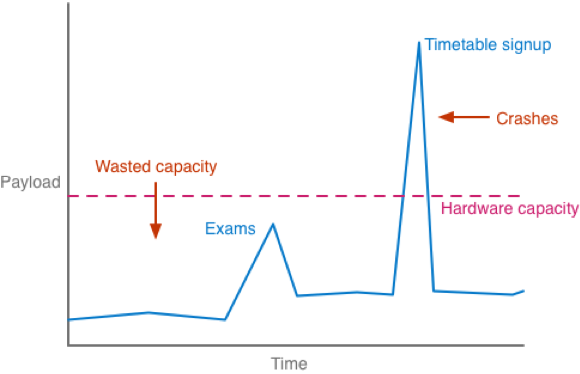
\includegraphics[width=3in]{CloudComputing_1.png}
\caption{Use of information system with fixed hardware capacity \label{fig:1}}
\end{figure}

Cloud computing would resolve this problem by scaling up for a couple of hours, and it would save money by scaling down during semester when the system is not used too heavily. Such cloud is called platform as a service.

Another cloud solution would be using an existing academic system, available as a service, where hosting is handled by the company that sells the system. 

\subsection{Infrastructure as a service}

Infrastructure services deliver computer hardware as a service. Clients, instead of having to purchase the infrastructure, pay regular fee to the provider to get scalable infrastracture.

An example of platform as a service is Amazon EC2:

\begin{quotation}
Amazon Elastic Compute Cloud (Amazon EC2) is a web service that provides resizable compute capacity in the cloud. It is designed to make web-scale computing easier for developers. \citep{amazon}
\end{quotation}

\subsection{Platform as a service}

Platform as a service is a whole platform moved to the cloud. 

\begin{quotation}
PaaS solutions are development platforms for which the development tool itself is hosted in the cloud and accessed through a browser. With PaaS, developers can build web applications without installing any tools on their computer and then deploy those applications without any specialized systems administration skills. \citep{paas}
\end{quotation}

An example of PaaS is Google App Engine.

\begin{quotation}
App Engine offers fast development and deployment; simple administration, with no need to worry about hardware, patches or backups; and effortless scalability. \citep{google_appengine}
\end{quotation}

\subsection{Software as a service}

Probably the most popular type of service cloud is software as a service. It’s a new model of selling software: Instead of selling individual versions, the provider hosts software and user data, giving user access from anywhere.

Hosting is usually outsourced to infrastracture provider, as described in previous sections. 

\section{Motivation}

During the last couple of years a lot of software has migrated from desktop application to web applications.

Many tasks can be now performed using only the web browser. A project called Chromebook \citep{chromebook} introduced a laptop which contains only a web browser and all the work is done using web applications.

That makes development and use of software better in many ways: Web applications are faster to implement, it’s easy to customize interfaces, there is no such thing as software updates anymore, and the data are stored and processed by the server.

When the data are stored on the server, they are stored more safely than on user's hard drive. It also allows data sharing and communication between users.

\subsection{Client applications}

\begin{figure}[ht!]
\centering
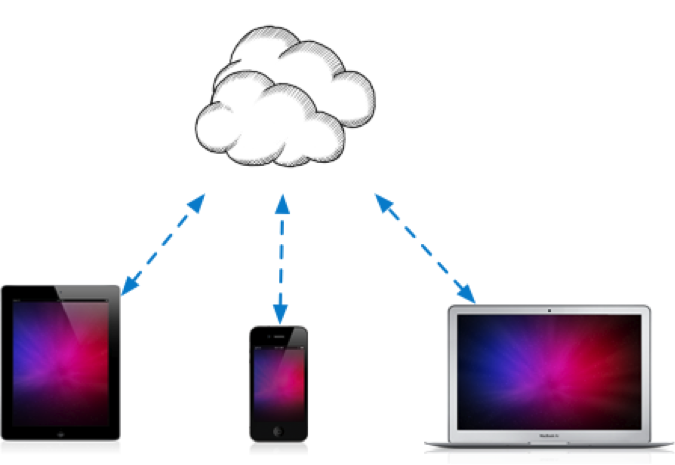
\includegraphics{Motivation_1.png}
\caption{Diagram of clients in cloud architecture \label{fig:1}}
\end{figure}

In the cloud architecture, client is the device that connects to cloud. Client application is software that runs on client and communicates with the cloud service. In SaaS, the client application is often delivered in form of web application: User can access it using their browser.

However, a web application isn't always sufficient. For example, on iPhone platform, web applications are limited, they can’t access some hardware features, such as camera. Native applications support these features, and those can be installed via App Store. So a client application can either be a website, or it can be a native application that requires installation.

If there's a native application, in the SaaS business model is usually free: It charges for using the service, not for installing software. If user downloads the free application, but are not subscribed to the service, they won't be able to get past the login screen. 

Atmosphere tries to improve these client applications and make their development faster. The next sections will discuss the current state of client applications.

\subsubsection{Desktop applications}

With SaaS becoming a popular model for software business, companies started focusing less on desktop applications and more on web applications.

Developing for desktop takes more effort than developing for web, mainly because it's easier to support all platforms when building a web app. For companies it might not be worth building individual application for every platform.

Still there are some well-known SaaS products that provide a decent desktop application. A good example are the social networks. They have millions of users and they provide an API.

WIP

With millions of users and open API it is only logical that developers try to improve the experience by building a desktop applications. As for a particular example, Twitter has tens of desktop clients for all Windows, Mac and Linux platforms.

It seems that user experience is generally better with desktop application rather than web applications. The first reason is that the user interface is on the client side: That means there are no requests, there is no need for AJAX, only the data is transferred through the network. Some desktop applications even use local storage to cache the local data.

So the only problem left to solve is the very case when application doesn’t work with local data, but always makes networks requests, blocking the interface, needlesly making user wait. 

The desktop library of Atmosphere solves this problem by providing a library that extends local storage framework and adds transparent networking without interface blocking. 

One last type of desktop applications are those with purpose of notifying users of events. Should an event occur in a web application, the only way of immediately notifying user is via email. These emails tend to get very annoyoing after time, so user start creating filters that hide them from the inbox, which partly defies the purpose.

A better way of notifying users is to provide a desktop application they can launch and quit. Part of Atmosphere is the notification server which together with client libraries allow instant notifications for events that occured in the application. 

\subsubsection{Mobile applications}

Mobile applications became a very important part of any SaaS. It is time when many users own smartphones with constant connection to the Internet, and they expect every service to provide a mobile application, that would allow them to perform the basic  tasks using a simplified user interface. 

Mobile applications are usually a top priority when a new SaaS product is shipped. Regular, web-based product is unusable on a small mobile phone. A special, mobile version of the site could solve the problem, but compared to native mobile apps, these lack a great deal of responsiveness and speed.

Also, a native mobile application provides access to hardware-specific features, such as the the camera, GPS, the accelometers, multi-touch event handling, and others. 

So what problems do the mobile applications have. Ironically, it seems that these are most evolved. Compared to desktop applications, they are built a lot more frequently. Compared to web applications, they are much more responsive and faster. 

There is even an excellent framework RestKit [10] that allows building iOS applications based on REST web services. It also provides a way of caching retrieved data in a local database.

The only flaw of this framework is that it doesn’t support creating objects locally, when there’s no internet connection, and then synchronizing with the web service. Atmosphere solves this problem by tracking local changes all the time, no matter if user has internet connection or not, and synchronizing them with the web service when there is connection available.

Notifications are supported on mobile platforms in different ways. On iOS there’s a central notification system, that is managed by Apple infrastructure. The application is not responsible for managing open connection to receive notifications, instead when an event occures on the server side, it notifies the Apple notification service that then delivers notification to the client. This solution is superior to managing connection by every client connection individually. First, it saves the memory footprint, CPU usage, thus it saves battery life. Secondly, the code responsible for managing the connection is provided and well tested by Apple. Network programming is a very unstable, so it would take a lot of effort to come up with solution as reliable as Apple’s. 

Atmosphere won’t deal with push notifications in a way of receiving notifications when application is not active. But it will apply the same solution of updating objects as soon as they are changed on a different machine to mobile applications. 

\subsubsection{Web applications}

There is one significant difference between desktop/mobile apps and those that run in a browser. Native apps ship a package of client code that needs to be installed and run on the client platform. Web applications, in contrast, can run anywhere without any installation.

About the greatest issue with current web applications is that they are not really applications. Most of them is just a set of web pages and forms. Some use AJAX to make requests in the background, but there is still occasional page reload.

That requires most of the logic on the server side while only the results of requests are delivered to user. This concept is old and must be replaced by JavaScript-heavy client side applications that have their own logic, especially around views. They would make request only when necessary.

This thesis doesn’t explore all of the possible solutions of achieving this goal for there are many various options. Instead, Atmosphere assumes the developer has or is building a JavaScript application.

Moving logic to the client side is a great improvement itself. Still there are the same problems as mentioned before. For example, TaskDo (one of Atmosphere-based applications, that were build along with the framework), provides an easy way to access user’s tasks in Google Tasks. The simple interface consists of two screens: List of „task lists“ and list of tasks in the list.

Without Atmosphere, clicking on a task list would result in a few seconds wait for the tasks inside to load. With Atmosphere, the data is already cached locally, so opening a task list is instant. TaskDo and other applications are described in section Case Study.

The next problem with web applications is that there are no push notifications, unless the business domain explicitly requires them. (Such as a chat application, or a game.) For most applications, it’s not exactly necessary to update objects  in real time between users, but it would make the application better.

\subsection{Conclusion}

It’s the current problems with client applications what Atmosphere is trying to remove. This section discussed what are the problems that make current client applications inconvenient to use and slightly outlined the proposed solutions. In further sections we’ll discuss the technologies that will be used and the solutions themselves.

\section{Technologies}

\subsection{HTTP and REST}

HTTP (Hypertext Transfer Protocol) is one of the basic protocols of the World Wide Web. HTTP implements the request-response and the client-server model. Take example of user navigation to search engine. In such case, the user's web browser is the \textbf{client}, and the computer where search engine is stored is the \textbf{server}. Typing the URL and hitting return key creates a \textbf{request} which is sent to the server over HTTP. Server processes this request and generates a \textbf{response}. The response is sent back to client (the user's browser) which processes it and presents data to user.

The request message is a short message containing the following: Method, path, headers and optional message body. Before we can discuss REST, it’s important to remind all HTTP methods. (GET and POST are the common ones, because they are supported by all browsers.)

Representational state transfer, or REST, is a style of architecture for HTTP interfaces. It's basic idea is that every object is represented as a resource. Actions can be performed on resources, such as index (will return list of all objects for specific entity), create (will create new record for entity), update (will update parameters of record) and delete (will remove a record). In REST, these actions are mapped to method and URL pairs. \citep{rails_way}

Atmosphere will act as client in the REST architecture. It will expect the source to be a RESTful HTTP interface, but still configurable. 

\subsection{HTML5}

Since Atmosphere relies heavily on HTML5 features, some of them will be described in this section. 

HTML5 is the new version of HTML with support for all kinds of new features. The following sections will go through these features, discuss their use and support in the web browsers. Also, we’ll discuss how these features fit with Atmosphere and what use they can be made of.

Before it would be worth mentioning that by using HTML5 there is increased chance that the application won’t work correctly, or won’t work at all for some users. In a good application, users with old browsers would be informed about this and not allowed to use the application at all, instead of leading them into thinking the issues are caused by the application. 

Can be this problem solved in a more elegant manner? Is there any solution that would bring bring the new features to users with old browsers? That depends on what feature it is. For example, if the browser doesn’t support WebSockets (which is a real situation – Android web browser doesn’t support it.), then the push notifications should be disabled, but the application should work without them. That is of course the case if the application is not completely based on WebSockets. Atmosphere applies this concept of graceful degradation: If the WebSocket support is not present, it simply won’t be used, but the application will still work through the REST interface as normal.

That was an example of degradable feature, there are more fundamental ones that simply require support. In that case there is no other solution than demanding user to upgrade their browser.

Another interesting solution is to bundle the application along with a modern browser and distribute it as a desktop application.

\subsubsection{CSS3}

CSS3 allows advanced styling of interface elements without use of images. The main advantage is being able to change looks later in the development process without having to use an image editor.

\emph{Animations} generally improve user experience by visualizing the action performed by the user. With CSS3, animations can be rendered using JavaScript. That means, instead of computing properties for each frame of animations, it is the responsibility of web browser to render it. Some browsers use GPU to accelerate these animations, which makes the interface feel much more like a native application. 

\emph{Border radius} is a simple feature that allows rendering elements with a border radius. 

\emph{Shadows} allow rendering shadows as if cast by text (text-shadow) or a some element (box-shadow.) 

\emph{Flex box} is a feature for creating „flexible“ boxes, that means making elements automatically expand to some part of the screen. It allows building interfaces, that looks like native user interface instead of web page. The original solution was mostly absolute positioning or JavaScript that would automatically reposition elements whenever the window was resized. 

\emph{Font face} allows using custom fonts and is already widely used. There are services, such as Typekit or Google Web Fonts, that let developers use any font from their collection by simply including short stylesheet in the page. 

\emph{Gradients} allow styling elements with gradients without having to use images.

Atmosphere doesn’t directly require any of these features as it is not working with the interface directly.  

\subsubsection{Geolocation}

Some HTML5 browsers support geolocation – a programming interface that lets web application request current location of the user, after user allows the application to access it. It is easy to gracefuly degrade when this feature is not available.

It is available on most of the mobile devices. 

Atmosphere doesn’t use this feature in any way.

\subsubsection{Canvas}

Canvas is a HTML5 element that allows dynamic rendering of vector objects and bitmaps. It is commonly used in graphic applications.

It is supported in all browsers, except Internet Explorer supports it only from version 9.0.

Atmosphere doesn’t use the canvas element.

\subsubsection{WebGL}

WebGL is a JavaScript extension that allows generation of interactive 3D graphics by sending instructions directly to GPU. It’s based on OpenGL ES 2.0. 

In supported browsers, WebGL is automatically enabled if user hardware is compatible. WebGL is  supported in version 9.0 and newer of Google Chrome, 4.0 and newer of Mozilla Firefox, 5.1 and newer of Safari (altough Safari has WebGL disabled by default.) As of time of writing, it is not supported by Internet Explorer. 

Atmosphere doesn’t use this feature either.

\subsubsection{Audio}

Audio is an element that is used to play sounds in web browsers. Before HTML5, this task was usually handled by embedding Flash file. 

Audio has been around for longer than other features and is currently supported by all major browsers.

\subsubsection{Local Storage}

Local storage is the one feature that used to make desktop application superior to web application in many cases. In the years 2000 to 2009 there have been many attempts to somehow add local storage to web applications. These include userData of Internet Explorer (part of DHTML Behaviors), Local Shared Objects of Adobe Flash and bridges with JavaScript, and SQLite databases provided by Google Gears.

HTML5 brings a new feature, Local Storage or sometimes called Web Storage. Websites can store up to 5MB of data in key/value pairs and even more after demanding user’s permission. Local Storage is supported by all major browsers, including Internet Explorer from version 8.0. It is also supported on mobile browsers, both Android (2.0 and up) and iPhone (2.0 and up.). 

Local Storage is thus a reliable way of storing application data on the client side. Atmosphere uses it to store local objects. 

\subsubsection{WebSQL and IndexedDB}

Simple key value storage is a good solution for simple applications. But sometimes greater flexibility is required. In desktop application such cases usually employ SQLite database, or other SQL based database solution. 

There are two solutions for the web: First one is WebSQL, which is similar to Google Gears a JavaScript interface to SQLite database. Such solution provides enough flexibility to store data in a more sophisticated manner than simple key value storage.

Unfortunately, WebSQL is not supported by Internet Explorer or Mozilla Firefox. This is not a result of slowness in development, Mozilla has stated they are not planning to support WebSQL. \citep{mozilla_indexeddb} Also, in 2010, W3C announced that WebSQL is a deprecated specification. \citep{w3c_webdatabase}

There is another solution, IndexedDB, which differs from WebSQL in API. Instead of writing SQL requests manually, it provides a JavaScript API to manipulate objects. Mozilla has implemented this database in version 4.0 of Firefox, it is also partially supported by Google Chrome 11.

Since not of these database is fully supported, Atmosphere doesn’t use either. Instead, applications should execute complicated database requests on the server and use REST API to retreive a subset of resources relevant to the user thus minimalizing complexity of client-side database requests making key-value storage sufficient.

Client-side SQL databases will be an interesting solution, and as they become a feature that’s supported on all platforms Atmosphere will try to use them. Until then we’ll stick with Local Storage.

\subsubsection{Websockets}

WebSockets is an extension of HTTP protocol. WebSockets hide the low level networking to provide simple API for connecting and sending simple text messages. 

WebSockets are most commonly used in web browsers, but not limited to. There are client libraries in languages such us Objective-C or Java, so they can be used in native iOS or Android applications.

The server part can be written in any language. There are servers written in Ruby, PHP, Java and others. But there is one server side environment that is favorite amongst many developers who use WebSockets. It’s Node.js, the environment that uses JavaScript as server language. Thanks to Node.js it’s possible to write server and client side for WebSockets in the same language with very similar API.  

WebSockets are supported in all current version of browsers. For Atmosphere, that would suffice, because the application can work without WebSockets, it would gracefully degrade to work without notifications. There are of course countless web applications that are based on WebSockets, that couldn’t work without them. There’s a library for this very purpose: Socket.IO. \citep{socketio}

\begin{quotation}
Socket.IO aims to make realtime apps possible in every browser and mobile device, blurring the differences between the different transport mechanisms. It's care-free realtime 100\% in JavaScript. \citep{socketio}
\end{quotation}

The idea behind Socket.IO is to use WebSocket when available and gracefully downgrade to other workarounds for push notifications in the brower. These include Flash file bridged with JavaScript, AJAX long polling and others. To use Socket.IO, a library needs to be included on both client and server side. With Socket.IO library the server side is expected to be written in JavaScript on Node.js, but there are other third party libraries that work in other environments.

Atmosphere uses Socket.IO which allows for notifications to work practically in any browser. (Internet Explorer 5.5+, Safari 3+, Google Chrome 4+, Firefox 3+, Opera 10.61+).

\subsubsection{Cache Manifest (Offline Applications)}

Cache Manifest is a feature that allows accessing a web application without active network connection. In order to implement cache manifest, a list of all resources that application require to work must be create and exposed using the cache manifest API. This will cause browser to store the resources for offline usage.

One of the effects is that the next time the web application is used, these resources will be loaded locally making the web application load instantly.

Using cache manifest also allows web application to be used offline without any internet connection at all. Atmosphere makes this possible by storing all objects locally. When user alters an object, it’s only marked as changed and pushed to the server the next time internet connection is available. 

By using both cache manifest and Atmosphere it’s possible to build web applications that simply work offline. 

\subsubsection{Conclusion}

Features listed here hardly include all of the ever evolving features of HTML5. We focused on the clue feature for Atmosphere, but we mentioned most of the features that could help building a next generation web application.

\subsection{PhoneGap and MacGap}

\begin{quotation}
PhoneGap is an HTML5 app platform that allows you to author native applications with web technologies and get access to APIs and app stores. PhoneGap leverages web technologies developers already know best... HTML and JavaScript. \citep{phonegap}
\end{quotation}

PhoneGap is a platform for wrapping HTML5 application into native packages. MacGap is an extension of PhoneGap that allows doing the same with desktop applications. MacGap works only on Mac computers.  There is a couple of interesting consenquences of using these platforms.

The first one is obvious. PhoneGap allows accessing native features of the device with JavaScript API. This connection is made using bridge between native code and UI element responsible for displaying the web page. (Usually called a WebView.) It’s possible to use some native features, such as accelometer, camera or compass. Lower level features are available too: Files, media, storage, notifications. 

Second is related to the way user perceive software. They are used to web applications being slow, laggy and unresponsive. Native applications, on the other hand, they perceive as fast and easy to use. Today it’s possible to build apps based on HTML5 (if built correctly), that are almost as good as native apps. When users are aware that they are dealing with a web application, not a native one, they expect the application to be slow and unresponsive, like they are used to with almost all web applications. 

Disguising a well-made web application as a native application may result into user believing they’re working with a native app, especially when the user is not too technical.

A great example is recently released LinkedIn iPad application of which 95\% is built with HTML5 instead of native technologies. (Shown in Figure \ref{fig:linkedin}.) \citep{linkedin_ipad}

\begin{figure}[htbp]
  \centering
    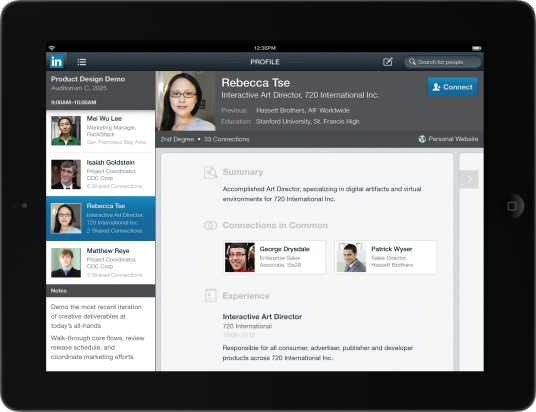
\includegraphics[height=3in]{figures/LinkedIn_iPad.jpg}
  \caption{LinkedIn iPad application}
  \label{fig:linkedin}
\end{figure}

The last reason is the ability to publish application in the App Store or Android Market. For Apple platform, App Store is the only way to distribute software (except for jailbroken devices.) For Android platform, it is possible to install applications from other sources than the Market, but in both cases having an application exposed in the App Store/Market helps uses find it, and increases downloads or sales.

Atmosphere doesn’t use these platforms in a direct way, but developer is encouraged to use them. 

\subsection{Cocoa}

Cocoa is a platform for developing Mac desktop and iOS mobile applications. The implementation of Atmosphere includes libraries for this platform.

Cocoa allows building native application using the Objective-C language and a tool called Interface Builder. This two allow developer to instantiate objects and graphically layout interface elements. All of the objects are then archived, frozen in place. When the interface file is loaded, the contents are unarchived, but not instantiated.

Cocoa provides basic elements to build both desktop and mobile applications. On desktop, forms elements, tables, collections and others are available. Mobile version contains different views made for touch devices. Also, the mobile version is extended by the touch framework for recognizing touch gestures, and other features specific for mobile devices.

Organization of code is usually done within the MVC pattern. For the model layer there is the Core Data library, that acts as peristance framework. The desktop version of Cocoa supports data bindings that automatically upate interfaces elements according to changes to models. This feature significantly reduces glue code in the controllers.

Another  very common pattern used by Cocoa is the observer pattern. There is notification center object, usually one for the application, which any objects can use to subscribe to notifications, or post notifications to. 

Core Data library persists special objects called managed objects into file or a database.  It manages attributes and relations of objects. Core Data uses fixed data schema which can be defined using a file or programatically. This is different from HTML5 as Core Data objects have fixed schema, and HTML5 are just objects serialized into key value storage. With Core Data it is of course possible to write more complicated applications with more complicated requests, because it can use SQLite as storage mechanism.

Atmosphere library sits on top of Core Data and adds automatic networking. Fetching or synchronizing objects can be triggered manually, or by watching  for changes using the notification center. (Observer pattern.)

Cocoa is a very deep framework with many features. This section is just an introduction to basic concepts and features that are later utilized by Atmosphere. 


\section{Design}

\subsection{Approach}

This chapter describes the high level design of Atmosphere platform, while the implementation details are described in later chapters. 

So far the thesis discussed the issue of current client applications. The conclusion is that interface blocking during network requests is one of the issues that could be solved.

\subsubsection{Asynchronous interfaces}

This section defines the term asynchronous user interface. \citep{maccaw_async}

In computer science, an asynchronous operation is such one, that does not block the caller while being processed, instead it returns immediately. It can be passed a callback that is called when the processing is finished.

Asynchronous interface is the result of applying the same concept to users and interfaces. The idea is to minimize amount of interface blocking. (Displaying some graphic that informs user the program is doing some work.)

An asynchronous interface gives immediate response, processing is done in the background and as soon as it is finished, the interface might present further results if needed.

\subsubsection{Local Storage}

\begin{figure}[ht!]
\centering
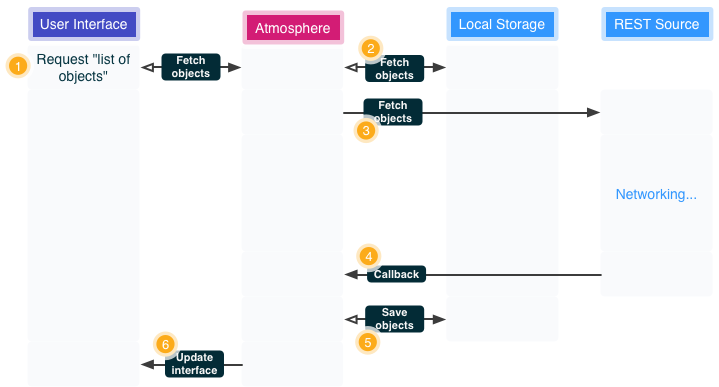
\includegraphics[width=430pt]{LocalStorage1.png}
\caption{Fetching objects using Atmosphere \label{fig:1}}
\end{figure}

The first step to achieve an asynchronous interface is storing some of the application data locally.

Figure \ref{fig:1} presents a situation of fetching a set of objects. When user tries to access a set of objects, \raisebox{-2.5mm}{
\includegraphics[height=0.3in]{Item1.png}} the application will first attempt to retrieve them from local storage, \raisebox{-2.5mm}{
\includegraphics[height=0.3in]{Item2.png}} which is an instant operation. User is provided with some data in zero time.

And the same time the application makes a network request to retrieve the newest data. \raisebox{-2.5mm}{
\includegraphics[height=0.3in]{Item3.png}} When the data is retrieved from the server, \raisebox{-2.5mm}{
\includegraphics[height=0.3in]{Item4.png}} Atmosphere will look at their unique identifiers and try to find an existing copy in the local storage. If the object is found, its attributes are updated and it is saved back to the local storage. If it is not, a new object is created locally. \raisebox{-2.5mm}{
\includegraphics[height=0.3in]{Item5.png}}

The user interface is bound to the local data. When new local data are saved, it is automatically updated to reflect current local data. \raisebox{-2.5mm}{
\includegraphics[height=0.3in]{Item6.png}}

\begin{figure}[ht!]
\centering
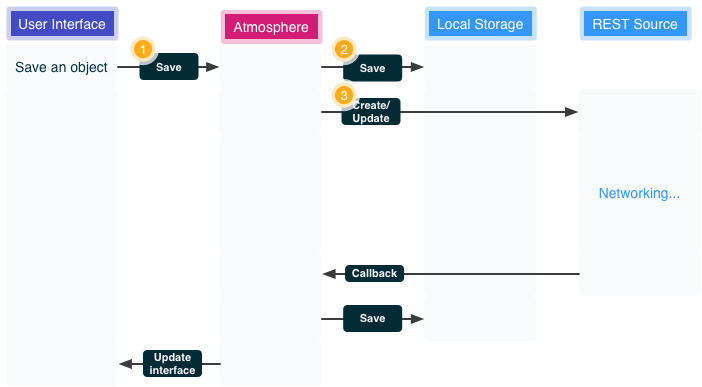
\includegraphics[width=430pt]{LocalStorage2.png}
\caption{Creating objects using Atmosphere \label{fig:2}}
\end{figure}

For making changes the objects, the workflow is similar, depicted in Figure \ref{fig:2}.

When user makes changes to an object, \raisebox{-2.5mm}{
\includegraphics[height=0.3in]{Item1.png}} the changes are immediately written to the local storage. \raisebox{-2.5mm}{
\includegraphics[height=0.3in]{Item2.png}} This operation is instant, so user sees response without any blocking. Now the object is marked as ``changed locally'', which schedules it for synchronization. The synchronization module picks it up, and sends it to the server. \raisebox{-2.5mm}{
\includegraphics[height=0.3in]{Item3.png}} The rest of the process works in the same way as with fetching objects.

Since the REST services have different actions for creating new objects and updating existing ones, it is important to decide whether to send a ``create'' or an ``update'' request. For this purpose Atmosphere keeps track of boolean information which indicates whether the object is ``local only''. This value is set true at the first time object is created, and is changed to false once confirmation about creation is received from the server.

Also, local objects need to be identified somehow. When an object is created locally, it is assigned a temporary identifier in form of UUID. Once it is successfully created remotely, the identifier is updated to permanent identifier assigned by the server.

\subsubsection{Recovering from failure}
\label{sec:failure_recovery}

Synchronization relies on network requests and network connection might be very unreliable at times. Also we have to consider that many of Atmosphere-based applications are developed especially for mobile devices and mobile connection is even less reliable.

The case of fetching objects does not require much attention. If objects fail to load, user will not see them. A notification about network failure can be displayed, but this is responsibility of application logic.

The case of saving object is more complicated. Atmosphere is designed in a way that it will always create a local object first. If the remote request fails, the local object exists, but the remote does not.

This problem is partly solved by keeping track of which objects are ``local only''. (See Figure \ref{fig:recovery1}.) Every object is marked as ``local only'' for as long as its existence was not confirmed by the server. \raisebox{-2.5mm}{
\includegraphics[height=0.3in]{Item1.png}} If one request fails, \raisebox{-2.5mm}{
\includegraphics[height=0.3in]{Item2.png}} the ``local only'' mark remains on object, \raisebox{-2.5mm}{
\includegraphics[height=0.3in]{Item3.png}} and the synchronization is attempted in the next cycle. \raisebox{-2.5mm}{
\includegraphics[height=0.3in]{Item4.png}}

\begin{figure}[htbp]
  \centering
    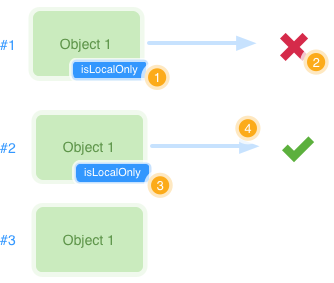
\includegraphics[height=2in]{Recovery1.png}
  \caption{Recovery from failure by keeping track of local objects}
  \label{fig:recovery1}
\end{figure}

A more complicated situation is when the network request is made, processed by the server (therefore the object is created), but the response never makes it back to the client. The object is created remotely, but the client application is not informed about this, so it never removes the ``local only'' mark. Then it tries to create the object again, because the mark was not removed and that results in two objects of the same attributes being created.

A possible solution is assigning permanent ID on the client side. Such solution would expect server to take ID as an argument to the create request.

Now a new object is created on the client side, it is assigned a temporary ID. Then it is sent to the server and server creates object with that ID. The response never comes back to the client, so client makes another create request, with the same ID. Server declines to create another object with the same ID, so it returns a confirmation message for existing object. This time client receives the confirmation message, so the object is marked as not local only.

This solution is not implemented by Atmosphere because it takes server side logic and Atmosphere is purely client-side framework. Implementing such a solution in fact takes only minor modification on server side, and is implemented by Edukit, as described in section \ref{sec:edukit}.

\subsubsection{Exceptions}

Always storing data locally whenever a new object is created might be harmful in certain cases.

For example a web commerce site might provide actions for adding products to the cart, and it might provide an action for submitting the order.

The programmer would probably decide to let Atmosphere manage creation of cart item object. But for order submission, it is better to block user interface, because users want to be sure everything worked. Doing such operation in the background might also lead users into thinking their order was submitted while it was not.

For this purpose, Atmosphere implementations provide a way to create or update an object using a synchronous (in terms of user interface blocking) request. 

\subsubsection{Other solutions}

There are simpler ways of achieving asynchronous interface.

One of them would be to create transient objects that would represent remote objects and still hide networking from the user. Such solution would be less complex because there would have to be no synchronization.

 One drawback would be that opening application for the first time would be slow as user would have to wait for network request to complete. 

Another reason to use local storage and synchronization is that the application can be used offline.

\subsubsection{Notifications}

\begin{figure}[htbp]
  \centering
    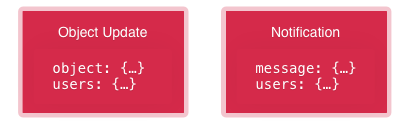
\includegraphics[width=3.5in]{figures/Notifications.png}
  \caption{Types of Atmosphere notifications}
  \label{fig:figures_NotificationServer}
\end{figure}


Atmosphere provides a WebSocket-based notification system for realtime updating of objects. The source application can use this system by making HTTP request to the Atmosphere notification server. (More detailed description is in section \ref{sec:notification_server}.) There are two types of notifications.

The first type is called \textbf{object update}. It's used to propagate an object update to a subset of connected clients. Such message contains object's attributes and list of users to send the notification to. Sending the object update message will cause connected clients to update their local object with the new attributes sent by the server. Using bindings or some other technique, the user interface is updated and user sees the new attributes in real time.

The second type is called \textbf{notification}. A notification contains custom object to be passed to the connected clients. Similarly, it contains list of clients to send the message to. 

A notification message will forward custom object to specified users. The client application is responsible for parsing and processing such message. Atmosphere provides a way for application to subscribe to these notifications.

\subsubsection{Live updates}

Notifications themselves don't suffice in all cases. Take as an example an application where multiple users would like to edit one page together. Once a change is made by one user, a notification could be sent to other users containing the whole page object.

What happens if a page is very long? Sending the whole object would be infeasible. The solution for this problem is to send only the changes made, not the whole objects.

Doing that requires further processing on the server side, to avoid conflicts. This processing can be done using operational transformation. \citep{ot} Since the processing has to happen on the server side, a custom server logic is required. Adding custom server logic is unfortunately not possible for Atmosphere, because one of the design decisions was to support custom REST servers.

This issue could be solved in future by developing a custom extendable Atmosphere server, with support for operational transformation.

\subsection{Components}

\subsubsection{Client}

Client is the computer where Atmosphere-based application is running. It can be a web, desktop or a mobile application.

\begin{figure}[ht!]
\centering
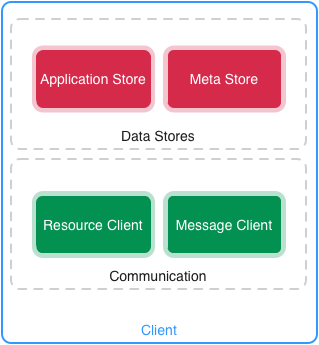
\includegraphics[width=200pt]{MainComponents.png}
\caption{Main components of the client \label{fig:3}}
\end{figure}

The implementations differ across platforms, but from a high level view there are two main component groups: One responsible for storing data locally and one responsible for communication with the HTTP server.

The Application Data Store is a component that is responsible for managing application objects. It is used for tasks like looking up an application object, or updating an application object. This component always depends on native way of storing data. In case of desktop applications, it depends on Core Data framework, etc. 

The Meta Store is a component that is responsible for storing meta objects, objects that encapsulate information that are needed by Atmosphere and that can be ignored by application itself.

List of meta data:

1. "is object changed" is a Boolean value that indicates whether the object was changed locally since the last synchronization. 

2. "is object local only" is a Boolean value that indicates, whether the object was retrieved from the server, or if it exists only in the local store. 

Components in the communication group are responsible for networking. Resource Client is component responsible for communication with the REST source while Message Client is responsible for communication with the Atmosphere notification server. 

\subsubsection{REST Source}

REST Source is an existing HTTP server. It is not important what language or technology is used to build this server, the only requirement for the server is to implement the basic CRUD methods: create, read, update and delete.

\begin{figure}[ht!]
\centering

\includegraphics[width=250pt]{RestSource.png}
\caption{Communication between the client and the REST source \label{fig:4}}
\end{figure}

The source can be also provided by a third party. For example, in application TaskDo (see section Case Study), the source is RESTful API of Google Tasks. 

Once the server is available and its methods are known, the client must be configured to use the correct methods to create, read, update and delete objects.

The communication between client and the REST source is then performed using HTTP methods.

\subsubsection{Notification server}
\label{sec:notification_server}

\begin{figure}[ht!]
\centering
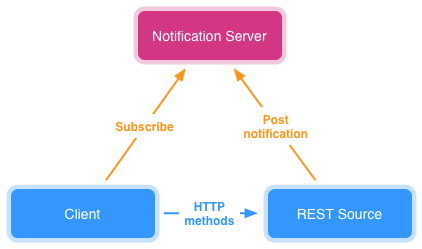
\includegraphics[width=250pt]{NotificationServer.png}
\caption{Use of the notification server by the client and the REST Source \label{fig:5}}
\end{figure}

Notification server is a component that stands between client application and REST source. Client subscribes to notifications on the notification server and the REST source posts notifications to the notification server. 

\section{Implementation}

This section starts by describing some important algorithms and implementation details of Atmosphere.

\subsection{Classes, data structures and algorithms}


This subsection describes data structures and algorithms used in JavaScript implementation. At the time of writing, the Cocoa implementation does not include all of the functionality described here.

\subsubsection{Data structures}

\textbf{URI} is a structure (in JavaScript implemented as object) which represents unique address of a local object. It consists of \textbf{entity} and \textbf{identifier}.

\textbf{Meta object} is structure which represents the meta information for an object. It contains the link back to the original object in the application store, and the values of meta attributes. Every application object managed by Atmosphere is assigned a meta object.

\subsubsection{Classes overview}

Both implementations provide object-oriented system of code organization. Components of Atmosphere are represented using classes as pictured in Figure \ref{fig:1}.

\begin{figure}[ht!]
\centering
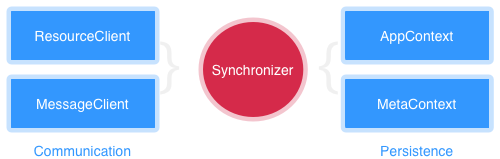
\includegraphics[width=350pt]{GeneralImplementation.png}
\caption{Classes used in implementation of Atmosphere \label{fig:1}}
\end{figure}


\subsubsection{Synchronizer}

Synchronizer is the main class of Atmosphere. It lies on top of other classes, and other classes use it to accomplish tasks. Its method can be divided into following groups.

\begin{enumerate}
\item Object lifecycle
\item Updating local objects with new data
\item Fetching objects
\item Saving objects
\item Making custom REST requests
\item Marking object as changed or synchronized
\item Synchronization
\end{enumerate}

\textbf{Object lifecycle} consists of class constructor, which initializes the class and all other required classes.

\textbf{Updating local objects} provides method for updating object specified by URI with new data. It also checks if updating data would change identifier of object, if so, then it updates the identifier in both application and meta context.

\textbf{Fetching objects} and \textbf{making custom REST requests} forward the call to resource client. These are only convenience methods. Similarly, \textbf{marking object as changed or synchronized} methods are forwarded to the meta context.

\textbf{Saving objects} allows specifying option which would make the saving 'synchronous'. In such case Atmosphere will immediately produce a save network request. When this option is set to false, the object is only marked as changed, and is synchronized in the next synchronization loop.

There are two purposes for this option: First, it disables offline usage. If the request fails, it will not be attempted again. Second, it is possible to pass options to such request. Note that asynchronous saving does not allow any options to be sent along with the save method. Making saving synchronous enables extra options, such as URL arguments or extra POST body.

\textbf{Synchronization} contains logic for looking up changed objects in meta context, deciding whether to send a create or update request, and finally calling the save method of resource client.

\subsubsection{Communication}

The communication layer consists of two classes: The resource client and the message client.

\textbf{Resource client} is used to download data over HTTP protocol conforming to REST style. In order to make a HTTP request, we need a URL for the resource. The process of converting a model and action pair to URL string is called routing. It is done by specifying an application specific routing table similar to one pictured in Figure \ref{fig:Routing}.

\begin{figure}[htbp]
  \centering
    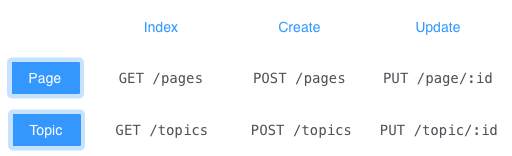
\includegraphics[width=300pt]{Routing.png}
  \caption{Example routing table for resource client}
  \label{fig:Routing}
\end{figure}

Once the correct URL is looked up in the table, the resource client prepends the base URL for the REST source, replaces occurrences of ID string with ID of record being saved, processes extra request-specific options and sends the request.

Resource client is also responsible for extracting data contained in the response returned from HTTP call. In the current implementation, only the JSON format is supported. Since the response could store data in many different ways (see Listing \ref{json}), Atmosphere allows setting custom function (or block in Objective-C) for retrieving these data from the JSON response.

\begin{lstlisting}[caption=Different formats of response JSON data,label=json]
// Simple JSON response
[{name: "Edukit"}, {name: "Atmosphere"}]
// More complicated JSON response
{"projects": [{"project": {name: "Edukit"}}, {"project": {name: "Atmosphere"}}]}
\end{lstlisting}

\textbf{Message client} is responsible for opening and maintaining connection over WebSocket. Both JavaScript and Cocoa implementations use Socket.IO \citep{socketio}, a pseudo-protocol implemented on top of WebSocket.

The typical update message contains object identifier and its data. The message client is responsible for updating the object with data contained in the message and it does so by calling appropriate method in the synchronizer class. Therefore message client remains a very lightweight class.

\subsubsection{Persistence}

\textbf{Application context} is class that manages application objects by providing methods such as create, update, change identifier or delete.

It's job is to unify interfaces of different model layers where Atmosphere might be used. In the current version, the only model layer is the one of Spine framework, but this class provides portability to other environments by encapsulating framework-specific model-related code.

\textbf{Meta context} manages meta information for each of application objects. It provides methods for finding meta objects for existing application objects, creating new ones, changing identifiers and updating meta attributes.

The motivation for this class came from the original implementation of Atmosphere which was intended only for Cocoa applications. Cocoa uses SQLite to store application objects, so it is not possible to dynamically add attributes to the schema.

Atmosphere needs some extra attributes, such as 'is changed' or 'is local only'. Therefore a new schema is used, where each item contains identifier of the application object and values for these meta attributes.

\subsection{JavaScript details}

\begin{figure}[htbp]
  \centering
    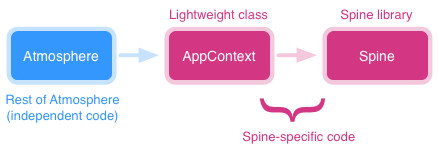
\includegraphics[width=3.5in]{Atmos-Spine.png}
  \caption{Usage of Spine by Atmosphere}
  \label{fig:figures_Atmos-Spine}
\end{figure}


At the time of writing, JavaScript implementation of Atmosphere is built on top of the Spine \citep{spinejs} library which is a lightweight framework for building JavaScript web applications.

The library does not completely rely on Spine, instead it only utilizes its model layer. Furthermore, all the code that requires Spine is contained in one small file (application context), which can be easily rewritten for other client side frameworks and their own model layers.

The implementation is written in CoffeeScript \citep{coffeescript}, which is a language that improves syntax of JavaScript by introducing many syntactic shortcuts such as semantic whitespace (inspired by Python) or accessing instance variables with the '@' sign. (inspired by Ruby).

The classes in persistence and communication layers implement the basic roles of Atmosphere, while the Synchronizer class is the entry point for working with Atmosphere.

The Spine integration contains shortcuts for calling Atmosphere methods directly from Spine models using the API users are already developers are already familiar with.

JavaScript implementation uses Socket.IO \citep{socketio} client library for opening WebSocket connections. The library enables socket-like functionality in browsers that don't support WebSocket using long-polling or Adobe Flash.

\subsection{Cocoa details}

The Cocoa implementation is packaged as Xcode framework. It is written in Objective-C and can be compiled for both desktop (Mac) and mobile (iPhone and iPad) platforms.

The Cocoa implementation relies on Core Data which is standard for storing objects in Cocoa applications. It binds onto Core Data workflow that allows automatically saving objects remotely as they are saved in the local storage.

\section{Use cases}

\subsection{TaskDo}

TaskDo \citep{taskdo} is a task manager application written using CoffeeScript \citep{coffeescript}, Spine \citep{spinejs} and Atmosphere. It features offline usage, synchronization with Google Tasks API \citep{google_tasks} and is bundled as application for Mac platform using MacGap. \citep{macgap}

The strong point of TaskDo is its close resemblance to native application. It's bundled as one, it's very responsive, but the most imporant thing is that it uses local data, which are synced with Google Tasks API using Atmosphere.

\begin{figure}[htbp]
  \centering
    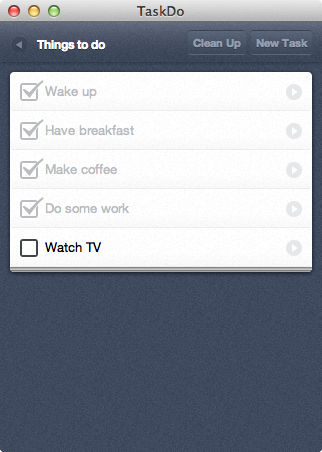
\includegraphics[height=3in]{TaskDo.png}
  \caption{Screenshot of TaskDo}
  \label{fig:taskdo}
\end{figure}

One of the problems during implementation was OAuth authentication. To successfully authenticate user, the OAuth2 protocol \citep{oauth} first requires redirection to provider's website. Then the user has to confirm that they want to share their application data with third party application. At the end of the authentication process the user is redirected back to the original application.

\begin{figure}[ht!]
  \centering
    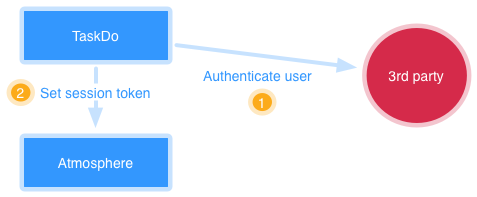
\includegraphics[width=3.5in]{TaskDoDiagram.png}
  \caption{Diagram of OAuth authentication}
  \label{fig:taskdo_diagram}
\end{figure}

Now the application is sent a session token, which has to be used with every subsequent API call in form of HTTP header.

Atmosphere provides a method for sending custom HTTP header with each request. TaskDo implements logic for completing the authentication process and then updates configuration for resource client to use the newly retrieved token with each request.

The Google Tasks API also returns JSON in a slightly more complicated format. For this reason, Atmoshere allows configuration of the way data are extracted from the response.

\subsection{Edukit}
\label{sec:edukit}

% \begin{figure}[htbp]
%   \centering
%     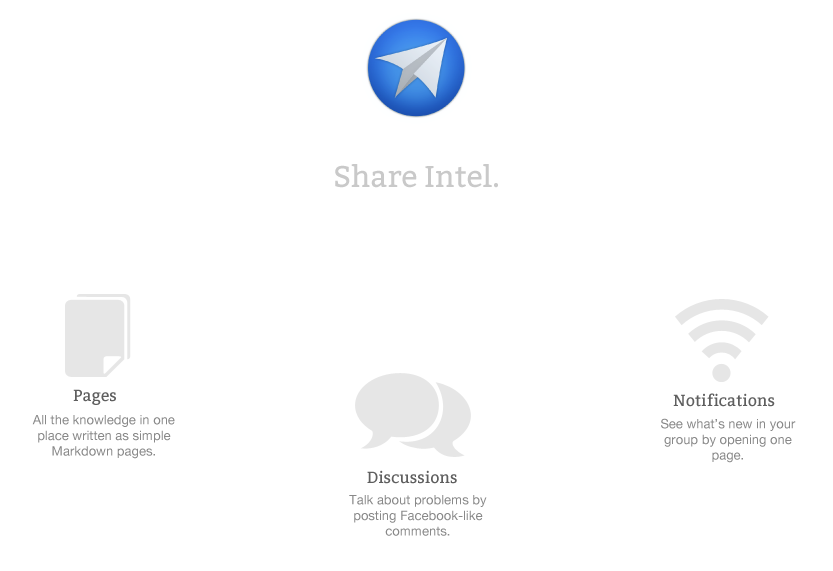
\includegraphics[height=3in]{Edukit.png}
%   \caption{The marketing diagram describing Edukit}
%   \label{fig:figures_Edukit}
% \end{figure}

Edukit is a data sharing platform intended for students. It features simple wiki-like pages, discussions and notifications. It helps students share and discuss knowledge. 

One of its key strengths is ease of use, the social aspect and the speed. Edukit is a very fast web application because of its minimal nature. But generating a new page with each action and delivering it to user can only be so fast. By using Atmosphere it was possible to go even further and make the application feel like a desktop application that provides instant response to almost every action made by user. 

\begin{figure}[htbp]
  \centering
    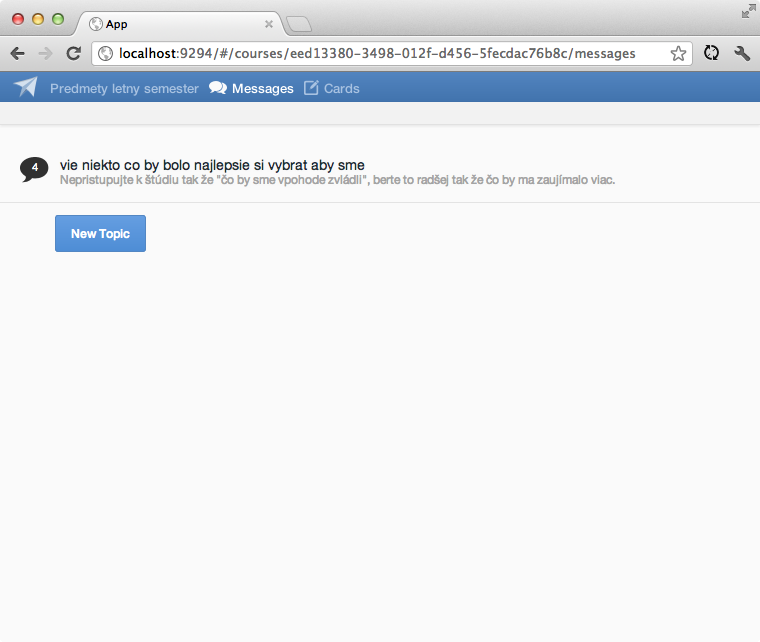
\includegraphics[height=3in]{EdukitScreen.png}
  \caption{Screenshot of Edukit showing list of topics in a course}
  \label{fig:figures_EdukitScreen}
\end{figure}

The new version of Edukit uses Spine.js and Atmosphere to create fully client-side web application, which stores data locally into the local storage of browser.

Atmoshere synchronizes these local data with the REST API of the original Edukit in the background. There are no changes in the original application involved, only exposing the REST API. The result is that it is possible to use both applications, the old and the new one at the same time.

\subsubsection{Real-time updates}

Edukit also utilizes the real-time notification server provided by Atmosphere as pictured in Figure \ref{fig:figures_EdukitMessages}. When a user creates a new message, a request is made against the original API written in Ruby. \raisebox{-2.5mm}{
\includegraphics[height=0.3in]{Item1.png}} The Ruby application collects information about the newly created message: its sender, contents and intended recipients. (All users that are in the course.) This information is then sent to Atmosphere notification server. \raisebox{-2.5mm}{
\includegraphics[height=0.3in]{Item2.png}} Atmosphere server now forwards the notification to clients connected via WebSocket. \raisebox{-2.5mm}{
\includegraphics[height=0.3in]{Item3.png}}

\begin{figure}[htbp]
  \centering
    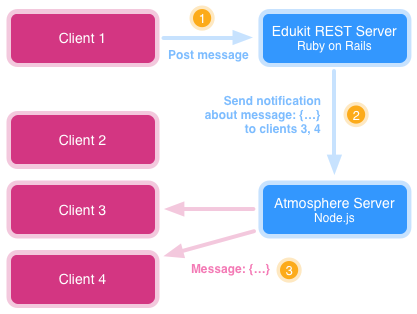
\includegraphics[height=2.5in]{figures/EdukitMessages.png}
  \caption{Posting messages with real-time updates in Edukit}
  \label{fig:figures_EdukitMessages}
\end{figure}


Since the Ruby application and the live notification server are running on the same machine, and the Atmosphere server is written in Node.js, there is almost no extra processing time for the original request. The result is ability to chat in real time with other users who are currently viewing the same topic.

\subsubsection{Failure recovery by using UUIDs}

Edukit implements failure recovery (see section \ref{sec:failure_recovery}) by using same object identifiers on both client and server side.

When a local object is created, it's assigned a new UUID. When it's synchronized, the server creates it in the database, and sets it's identifier to the one created on the client side.

This helps prevent the case of one local object being created two times on the server side in case of network failure. This situation can never happen, because server uses client identifier to create remote object, so if an object with same identifier already exists, it will simply return that object instead of creating a new one.

\subsection{Zone}

\begin{figure}[htbp]
  \centering
    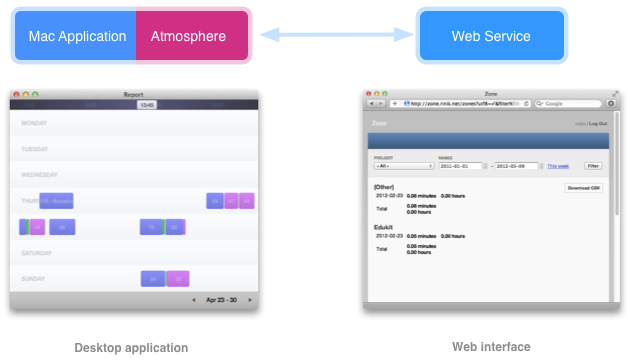
\includegraphics[height=2.5in]{figures/ZoneDiagram.png}
  \caption{Components of Zone}
  \label{fig:figures_ZoneDiagram}
\end{figure}

Zone is an application for Mac that allows simple time tracking. At its first iteration the mission was to help people focus on their work by "zoning in", which would make the toolbar icon purple, reminding user they're working.

At later iterations, a new feature was added: Overview of previous zones throughout the week. This feature would help users find their productive time of the day by letting them visualize how long they were able to focus without taking a break.

The last iteration added synchronization with a web service. Its web interface allows viewing zones, exporting them into PDF and generating invoices. The last iteration utilizes Atmosphere's Cocoa client library to synchronize local data about zones with the web interface.




\section{Other solutions}

During the time of writing many new projects were released. Some of them are very similar to Atmosphere, others target wider range of problems.


\subsection{Meteor}

Meteor \citep{meteor} is a whole JavaScript framework for building distributed, real-time JavaScript applications. First of all, it provides the environment for building JavaScript applications. This environment includes automatic template rendering based on model updates.

The problem with this approach is that if the developer already knows a UI framework, such as Spine.js, \citep{spinejs} they can either use Meteor instead, or figure out a way to connect the UI part of their framework and the data part of Meteor.

It provides a database-like API on the client side. Client-side code can manipulate objects in the application directly. Changes made to objects are propagated to other clients automatically in real-time using WebSockets.

The server side is written in Node.js and the documentation \citep{meteor_doc} doesn't mention any means of implementing custom logic on the server side. That, first of all, represents a security risk. The client makes changes directly to database objects. Client is written in JavaScript and since it is not a compiled language, it can be changed by user at any time. Therefore, client can change database objects directly, which can become an issue if application is used by multiple users.

Secondly, using this approach could result in unexpected state of objects in case of network failure. For example, single action may create two interdependent objects. If one of these requests fails, there is one object which depends on another objects, which doesn't exist.

If these two objects were created in a server procedure called using one request, it would assure that either both or none of the objects are created.

Meteor uses MongoDB to store its data. Meteor doesn't provide a library for Cocoa, or any other desktop or mobile platform. It is open-source and its source code is released under MIT license.

\subsection{Firebase}

Firebase \citep{firebase} is a product similar to Meteor. The key difference is that it doesn't provide a whole framework for building JavaScript applications, but only the data layer.

This allows using existing JavaScript applications written in other frameworks and adding Firebase data layer. The data binding is done by attaching callbacks to Firebase data layer. Existing application with its own custom UI logic first attaches a callback to be called when Firebase data changes, and then is notified of changes so it could display the current state.

Another difference between Meteor and Firebase is that Firebase requires users to use their hosting to store the data. It is not open source and it does not provide a way to self-host the data. It is founded by YCombinator \citep{ycombinator} and other angel investors. It also doesn't provide a library for other than web platform.

\subsection{Simperium}

Simperium is a project that is very similar to Firebase. It also doesn't provide a whole JavaScript framework, only data layer.

Similarly to Meteor and Firebase, Simperium provides real-time object synchronization. One very powerful difference is built-in operational transformation. \citep{ot} This allows sending only the portions of data that have changes which improves performance dramatically when dealing one larger objects. Also it adds automatic resolution of conflicts: If two users change one object, their both changes will be preserved.

Simperium also allows writing custom server logic. Programmers have to use the environment provided by Simperium. The server side hosting is still provided by Simperium. It is also founded by YCombinator \citep{ycombinator} and not open-source. 

Simperium also comes with a Cocoa framework for building iOS application. This framework adds feature of caching data for offline use. Interestingly, this feature is not provided for web applications.

\subsection{Comparison with Atmosphere}


\tabcolsep=10pt
\begin{table}[!hb]
  \centering
  \rotatebox{90}{
  \begin{tabular}{|p{2.5cm}|p{2cm}|p{3cm}|p{2cm}|p{3cm}|p{2cm}|p{1.5cm}|}\hline
                & Platforms             & Requirements            & Server                  & Real-time                       & Offline use         & Open-source \\\hline\hline
\textbf{Meteor}      & JavaScript                & Meteor UI framework     & Provided                & Yes                             &                     & Yes           \\\hline
\textbf{Firebase}    & JavaScript                & None                    & Provided                & Yes                             &                     & No            \\\hline
\textbf{Simperium}   & JavaScript, Mac, iOS      & None                    & Provided                & With operational transformation & Mac and iOS only    & No            \\\hline
\textbf{Atmosphere}  & JavaScript, Mac, iOS      & None                    & Any REST API            & Yes                             & Yes                 & Yes           \\\hline
  \end{tabular}
  }
  \caption{Comparison of solutions similar to Atmosphere}
  \label{table:comparison}
\end{table}


Atmosphere is very similar to Simperium by a few key points: It provides custom server logic, real-time synchronization, Cocoa library and an option for offline usage.

It is still very different from these frameworks in one aspect: It allows building applications that utilize and existing application with its REST API. All of the frameworks mentioned here require a whole new server-side application practically making developers rewrite their server code from scratch. (Or in worse case skip writing the server code.) Atmosphere is also open-source.

Because of this design decision Atmosphere cannot bring some features such as operational transformation for live editing. It would be impossible to implement it without drastically changing server code, which is one of the strong points of Atmosphere: It allows building real-time application with minimal change at the server side.

The overview of features provided by these projects is shown in Table \ref{table:comparison}.

%
%\section{Analytical considerations}

Text záverečnej práce obsahuje kapitolu, v~rámci ktorej autor uvedie
analýzu riešených problémov. Táto kapitola môže byť v~prípade
potreby delená do viacerých podkapitol. Autor v~texte záverečnej
práce môže zvýrazniť kľúčové slová, pričom sa použije príslušný štýl
pre kľúčové slová -- napr. toto je kľúčové slovo. V~texte môžu byť
použité obrázky a~tabuľky podľa nasledujúcich príkladov:

\begin{figure}[!ht]
\centering \unitlength=1mm
\begin{picture}(30,30)(0,0)
\put(0,0){\line(1,0){30}}
\put(0,0){\line(0,1){30}}
\put(30,0){\line(0,1){30}}
\put(0,30){\line(1,0){30}}
\end{picture}
\caption{Toto je štvorec}\label{o:1}
\end{figure}


Obrázok by mal byť podľa možnosti centrovaný. Pri jeho opisovaní
v~texte treba použiť odkazy na obrázok v~tvare Obrázok~\ref{o:1}.

\tabcolsep=8pt
\begin{table}[!ht]\caption{Prehľad jednotiek}\label{t:1}
\smallskip
\centering
\begin{tabular}{|l|c|} \hline
Názov	& (\,Jednotka v~sústave SI) \\ \hline
Napätie & $\upmu$V \\ \hline
\end{tabular}
\end{table}
\nomenclature{$\upmu$}{mikro, $10^{-6}$}
\nomenclature{SI}{Syst\`eme International}
\nomenclature{V}{volt, základná jednotka napätia v sústave SI}

Tabuľka by mala byť podľa možnosti centrovaná. Pri jej opisovaní
v~texte treba použiť odkazy na tabuľku v~tvare: pozri
Tabuľku~\ref{t:1}. Na číslovanie obrázkov, resp. tabuliek treba použiť
triedenie. Za slovom {\it Obrázok} nasleduje ako prvé číslo kapitoly
alebo časti, v~ktorej sa obrázok nachádza, potom medzera, pomlčka,
medzera a~poradové číslo ilustrácie v~danej kapitole alebo časti.
Napr.:~Obrázok~\ref{o:1} (čiže: prvý obrázok v~druhej kapitole alebo
časti). V~prípade, ak tabuľka presahuje stranu, je možné použiť balík
\verb+longtable+.

Navrhujeme zaraďovať obrázky v~elektronickej podobe. Napríklad
Obrázok~\ref{o:2}, ktorý opisuje riešenie diferenciálnej rovnice
tlmených oscilácií
%% \def\ud{\mathrm{d}}
\begin{equation}\label{r:1}
\frac{\ud^2y}{\ud t^2}+\frac{\ud y}{\ud t}+y =0, \qquad y(0)=1, \quad
y\,'(0)=15,
\end{equation}
bol vytvorený v~MATLABe a~príkazom \texttt{print tlmosc.eps -f1
-deps2} bol uložený vo formáte Encapsulated Postscript. Na prípadné
použitie pdf\LaTeX{}u sa obrázok konvertuje do formátu PDF, napr.
pomocou programu \texttt{epstopdf}. Zvyčajne sa číslujú vzťahy, na
ktoré sa v~texte odvolávame. Napríklad: vzťahy (\ref{r:1}) definujú
Cauchyho začiatočnú úlohu.


\begin{figure}[ht!]
\centering
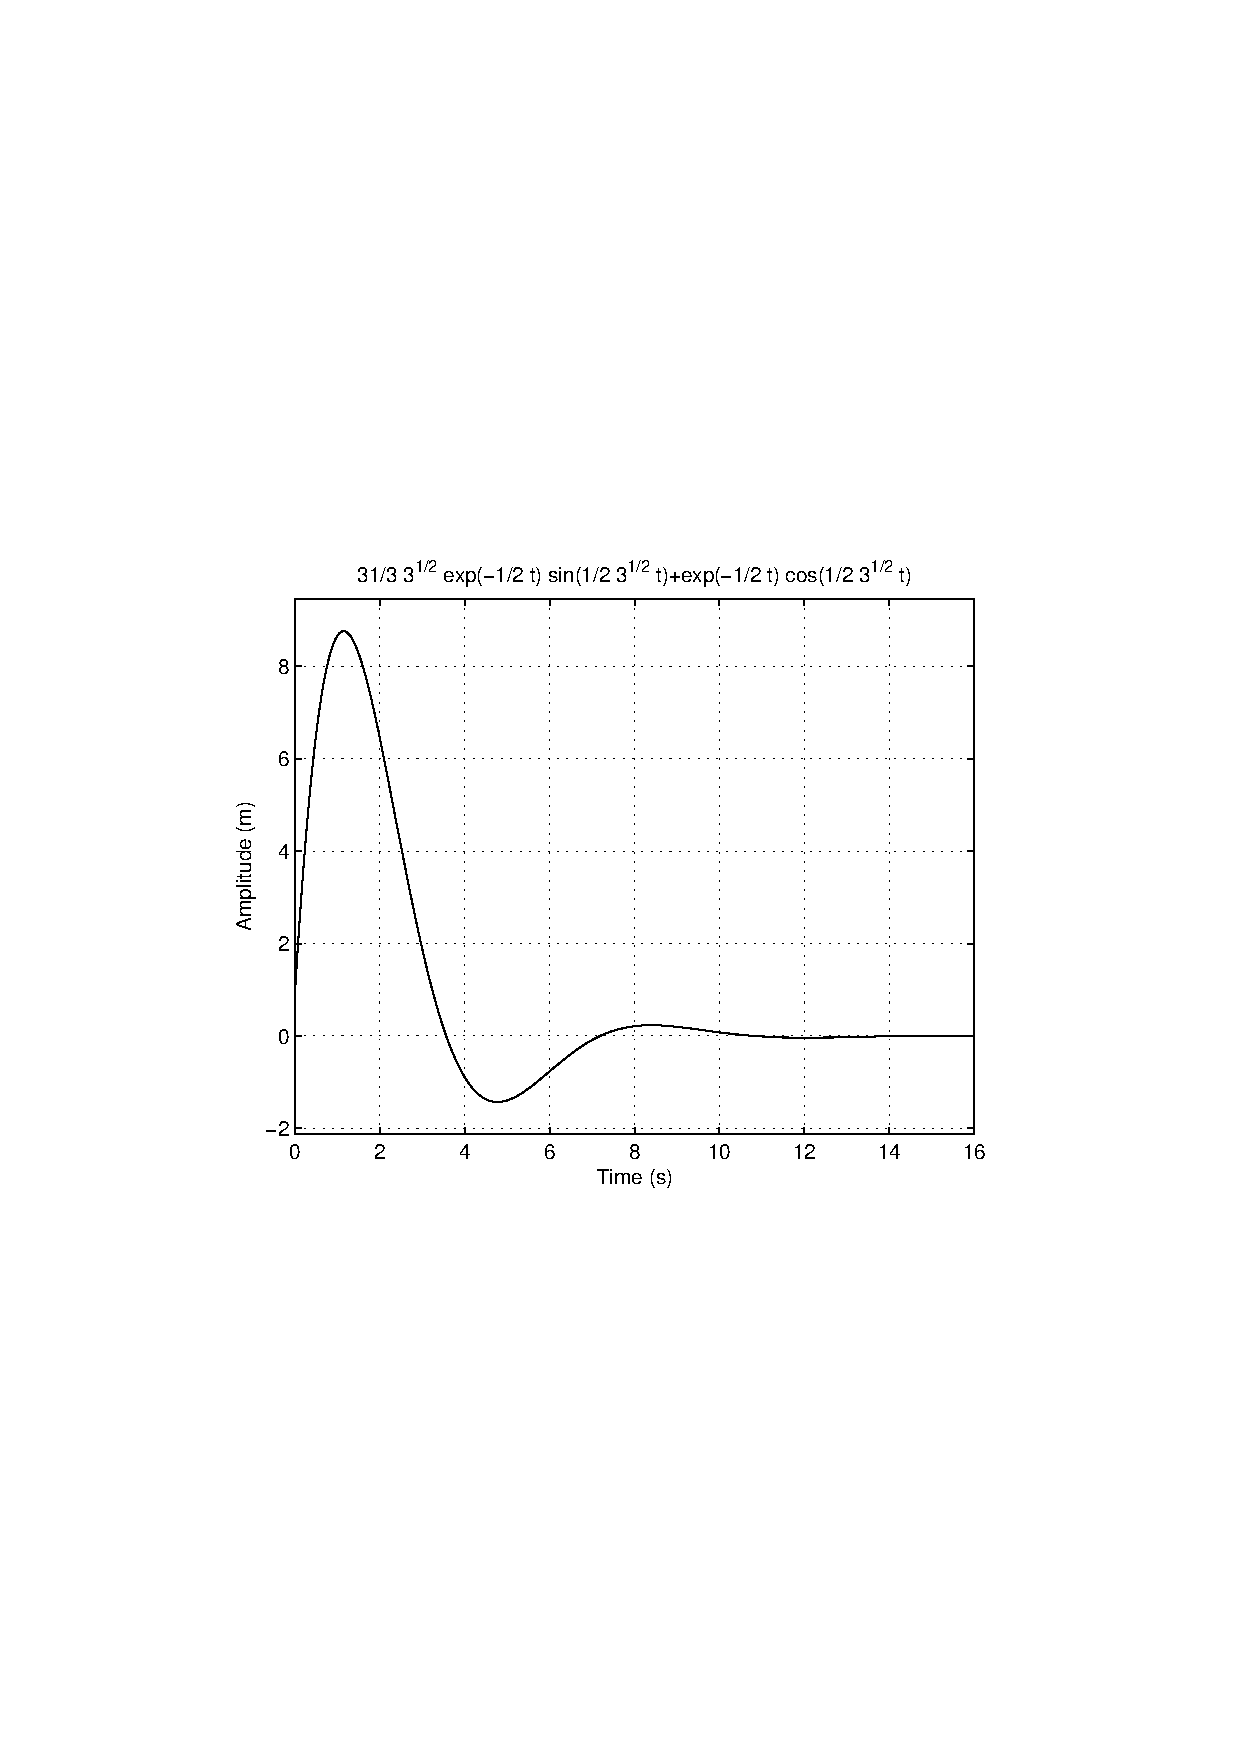
\includegraphics[width=0.7\textwidth]{tlmosc}
\caption{Grafické zobrazenie riešenia rovnice \ref{r:1}}\label{o:2}
\end{figure}



\subsection{Subsection}
Podkapitoly záverečnej práce majú za úlohu členenie textu záverečnej
práce s~cieľom, čo najväčšej prehľadnosti. Kapitol môže byť viacero
a~v~ich názvoch sa používa desatinné číslovanie.
%
%\renewcommand{\thesection} {\Alph{section}}
\section{Developer's guide}

\subsection{Introduction}

Atmos2 is a library that adds synchronization to models in JavaScript applications. 

Its goal is to make user interfaces very responsive by hiding the networking. 

\subsubsection{Overview}

\begin{figure}[htbp]
  \centering
    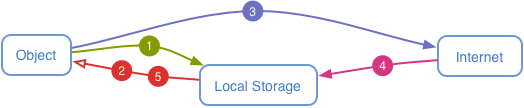
\includegraphics[width=4in]{figures/atmos-02.png}
  \caption{Overview of Atmosphere functioning}
  \label{fig:figures_atmos-02}
\end{figure}

\begin{enumerate}
\item Object is saved to local storage. 
\item User interface is immediately updated
\item Request is made to update the object on the remote side
\item Local version is updated from the response
\item User interface is updated according to changes received from the server
\end{enumerate}

\subsubsection{API Example}

\begin{lstlisting}[caption=Fetching objects from remote source,label=list1]
MyModel.sync(remote: true)
\end{lstlisting}

Code in Listing \ref{list1} fetches remote data and persists them in a local collection. Triggers an event on the model, so that the user interface could be updated.

\begin{lstlisting}[caption=Saving object,label=list2]
myRecord.save(remote: true)
\end{lstlisting}
    
Code in Listing \ref{list2} stores changes in local storage and makes remote request. When the request is done, it updates the local data and triggers event to update the user interface.

\subsubsection{Features}

\begin{enumerate}
\item \textbf{API configuration}: Advanced options of configuring API. So far used with typical Rails app and Google Tasks API.
\item \textbf{Fetching and caching}: Objects can be fetched and cached in local storage.
\item \textbf{Sync and posting}: When object is changed, it's saved locally, then posted to the server.
\item \textbf{Offline usage}: The design allows for building offline applications.
\item \textbf{Live updating}: Comes with [atmos2-server](https://github.com/vojto/atmos2-server) which is lightweight Node.js proxy for updating objects in real time.
\end{enumerate}

\subsubsection{Notes}

The current implementation uses the model layer of \href{http://spinejs.com}{Spine.js}. All the code that works with Spine is encapsulated in the AppContext class, which is 80 lines of CoffeeScript.

\subsection{Getting started with the JavaScript library}

Take existing Spine app or create a new one.

Install atmos2.

\begin{lstlisting}[caption=Installing atmos2 package]
git clone git://github.com/vojto/atmos2.git node_modules/atmos2
\end{lstlisting}

\textbf{Adding modules to slug.json}

Add these modules to your \texttt{slug.json}:

\begin{lstlisting}[caption=Updating slug.json with atmos2 package]
"dependencies": [
…
	"atmos2",
	"atmos2/lib/spine"
],
\end{lstlisting}

\textbf{Setting up the model}

Let's say this is your current Spine model:

\begin{lstlisting}[caption=Current Spine model]
class Task extends Spine.Model
  @configure 'Task', 'title', 'kind', 'selfLink'
\end{lstlisting}

\textbf{Extending the model}

All you have to do is require Atmosphere's Spine adapter, and extend model with it.

\begin{lstlisting}[caption=Requiring Atmosphere's Spine adpater]
require('atmos2/lib/spine')

class Task extends Spine.Model
  @configure 'Task', 'title', 'kind', 'selfLink'
  @extend Spine.Model.Atmosphere
\end{lstlisting}

Atmosphere will automatically use the local storage.

\textbf{Setting up the synchronizer}

Do this somewhere, where it will be executed before anything else.

\begin{lstlisting}[caption=Setting up the synchronizer]
Atmos = require('atmos2')

atmos = new Atmos
atmos.resourceClient.base = "https://www.googleapis.com/tasks/v1/users/@me"
\end{lstlisting}

As you can see, this example will work with Google Tasks API. But first, Atmosphere needs more information.

\begin{lstlisting}[caption=Setting up Synchronizer]
atmos.resourceClient.routes =
  Task:
    index: "/lists"
atmos.resourceClient.addHeader "Authorization", "OAuth #{token}"
atmos.resourceClient.IDField = "id"
atmos.resourceClient.dataCoding = "json"
atmos.resourceClient.itemsFromResult = (result) -> result.items
\end{lstlisting}
    
\begin{enumerate}
\item \texttt{routes} specifies path that will be hit on actions: index, create, update, delete. (TODO: Add others to the example.)
\item \texttt{addHeader} adds header to every request. In this case, we're adding OAuth Authorization, which we've taken care of someplace else, so we have a token.
\item \texttt{IDField} every retrieved object must have an ID. Some APIs expose this ID in field \texttt{id}, others \texttt{identifier}, so this settings lets you set it. If a record with empty ID will be retrieved, Atmosphere will throw an error.
\item \texttt{dataCoding} can be \texttt{form} or \texttt{json}, specifies in what format will be outgoing data encoding and sent. (Also, what \texttt{Content-Type} will be used)
\item \texttt{itemsFromResult} is a function that will be used to get the items from object decoded from response JSON. In this case, we receive a JSON that looks like this: \texttt{{items: [...]}}, so we need to tell Atmosphere how to look for actual records.
\end{enumerate}


\subsubsection{Fetching objects}

\begin{lstlisting}[caption=Fetching objects]
Task.sync(remote: true)
\end{lstlisting}

This will first fetch data from local storage triggering the \texttt{refresh} event, then make the network request, update local data, and trigger \texttt{refresh} event again.

\subsubsection{Saving objects}

\begin{lstlisting}[caption=Sending objects]
task = new Task({title: "Task 2"})
task.save(remote: true)
\end{lstlisting}

Calling \texttt{save} will first save the object locally, then it will make network request to save it again. \texttt{create} action will be used.

If you call \texttt{save} on already saved object, \texttt{update} action will be used. Atmosphere keeps track of all objects you saved with \texttt{remote} flag to differentiate between objects that have been sent previously and those once that haven't.

\subsection{Getting started with the Cocoa library}

\subsubsection{Installation}

Atmosphere for Cocoa is available as \href{http://cocoapods.org/}{CocoaPods} package. In order to install Atmosphere, your first need to enable CocoaPods for your project. For installation instructions please see the \href{http://cocoapods.org/}{CocoaPods} website.

Add Atmos2 to your Podfile.

\begin{lstlisting}[caption=Adding Atmos2 to your Podfile]
dependency 'Atmos2', {:git => 'git@github.com:vojto/atmos2-cocoa.git', :branch => 'master'}
\end{lstlisting}

\subsubsection{Setup}

The next step is to setup the synchronizer. In order to do that, open the main entry point for your application (usually the app delegate) and include Atmos2 header file.

\begin{lstlisting}[caption=Including Atmos2 header file]
#import <Atmos2/Atmosphere.h>
\end{lstlisting}

In your main class header file create a new instance variable that will hold reference to the synchronizer.

\begin{lstlisting}[caption=Adding instance variable for synchronizer]
@property (strong) ATSynchronizer *sync;
\end{lstlisting}

The next step is to set up the synchronizer.

\begin{lstlisting}[caption=Setting up the synchronizer, label=lst3]
self.sync = [[ATSynchronizer alloc] initWithAppContext:self.managedObjectContext];
[self.sync setBaseURL:@"http://localhost:6001"];
[self.sync loadRoutesFromResource:@"Routes"];
[self.sync setIDField:@"_id"];
\end{lstlisting}

The Listing \ref{lst3} shows very simple setup that first initializes a new synchronizer with current application context, sets base URL of the REST source, loads routing table from \texttt{Routes.plist} and finally sets up the ID field for parsing responses.

The routes file should contain a dictionary for each entity with keys representing actions and values representing HTTP actions in \texttt{method /path} format. An example routes file is portrayed in Figure \ref{fig:figures_routes-cocoa}.

\begin{figure}[htbp]
  \centering
    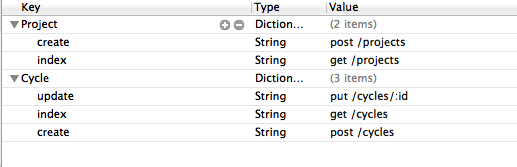
\includegraphics[width=4in]{figures/routes-cocoa.png}
  \caption{Example routes file}
  \label{fig:figures_routes-cocoa}
\end{figure}

\subsubsection{Fetching objects}

Listing \ref{lst4} shows how to fetch objects for an entity Project.

\begin{lstlisting}[caption=Fetching objects for an entity,label=lst4]
[self.sync fetchEntity:@"Project"];
\end{lstlisting}

Calling this command will fetch remote objects and store them locally. The application should be using data bindings or similar mechanism to update data when they change in Core Data store.

\subsubsection{Saving objects}

Saving objects is done automatically by watching changes in Core Data context. When an object is saved locally such as code in Listing \ref{lst5} shows, Atmosphere automatically sends it to the server.

\begin{lstlisting}[caption=Saving objects locally,label=lst5]
PLProject *project = (PLProject *)[NSEntityDescription insertNewObjectForEntityForName:@"Project" inManagedObjectContext:self.context];
project.title = @"New Project";
[self.context save:&error];
\end{lstlisting}
%
\section{Conclusion}

This thesis is focused on client applications for SaaS products. It starts by general analysis of these applications. The result is that there is still a lot of improvement space. Most of the applications require users to wait for network requests to finish, even when it's not needed. Also, only some of the application provide concurrent access by real-time data synchronization.

Once the problem is defined, the thesis continues by analyzing available technologies that could be used to solve it. There are many new HTML5 features such as WebSockets and local storage that could be used for building Atmosphere. Building desktop applications is a viable solution too.

The next part introduces the basic ideas behind the design of Atmosphere. It is concluded that the design should allow working with an external REST API, it should cache objects locally and synchronize them in background by keeping track of changed objects. A high-level structure of the libraries is outlined too.

The framework is implemented for two environments, the web (JavaScript) and Mac/iOS (Cocoa). The details of this work, such as specific data structures and algorithms are described in the next chapter. The rest of the chapter describes implementation specifics for individual platforms.

Next follows a brief description of how was Atmosphere used in three client applications for cloud services. The chapter contains real-world backing for some of the decisions made in the design phase, as well as description of new problems encountered while implementing these applications.

The work is concluded by comparing Atmosphere to other similar products. All of these products have existed for only a couple of months which shows that this area is in a very fast development.

%%
\begin{thebibliography}{999}
\addcontentsline{toc}{section}{\numberline{}{Bibliography}}

\harvarditem{Christopher Keene}{2009}{paas}
KEENE, C. 2009 \emph{What is Platform as a Service (PaaS)?}
  \newblock [Online, accessed 31.1.2012].
\url{http://www.keeneview.com/2009/03/what-is-platform-as-service-paas.html}

\harvarditem{Amazon}{2012}{amazon}
\emph{Amazon Elastic Compute Cloud (Amazon EC2.)}
  \newblock [Online, accessed 31.1.2012].
\url{http://aws.amazon.com/ec2/}

\harvarditem{Google}{2012}{google_appengine}
\emph{Google App Engine}
  \newblock [Online, accessed 31.1.2012].
\url{http://code.google.com/appengine/ }

\harvarditem{Mozilla}{2012}{mozilla_indexeddb}
\emph{Beyond HTML5: Database APIs and the Road to IndexedDB. }
  \newblock [Online, accessed 31.1.2012].
\url{http://hacks.mozilla.org/2010/06/beyond-html5-database-apis-and-the-road-to-indexeddb/}

\harvarditem{W3C}{2012}{w3c_webdatabase}
\emph{Web SQL Database.}
  \newblock [Online, accessed 31.1.2012].
\url{http://www.w3.org/TR/webdatabase/ }

\harvarditem{Socket.IO}{2012}{socketio}
\emph{Socket.IO: the cross-browser WebSocket for realtime apps.}
  \newblock [Online, accessed 31.1.2012].
\url{http://socket.io}

\harvarditem{PhoneGap}{2012}{phonegap}
\emph{PhoneGap}
  \newblock [Online, accessed 31.1.2012].
\url{http://phonegap.com}

\harvarditem{Alex MacCaw}{2012}{maccaw_async}
MACCAW, A. 2011 \emph{Asynchronous UIs – the future of web user interfaces.}
  \newblock [Online, accessed 31.1.2012].
\url{http://alexmaccaw.co.uk/posts/async_ui}

\harvarditem{Blake Watters}{2012}{restkit}
WATTERS, B. 2011 \emph{RestKit}
  \newblock [Online, accessed 31.1.2012].
\url{http://restkit.org/ }

\harvarditem{CoffeeScript}{2012}{coffeescript}
\emph{CoffeeScript}
\newblock [Online, accessed 1.5.2012]
\url{http://coffeescript.org/}

\harvarditem{Spine.js}{2012}{spinejs}
MACCAW, A. 2012 \emph{Spine.js}
\newblock [Online, accessed 1.5.2012]
\url{http://spinejs.com}

\harvarditem{Atmos2}{2012}{atmos2_github}
RINIK, V. 2012 \emph{Atmos2}
\newblock [Online, accessed 1.5.2012]
\url{https://github.com/vojto/atmos2}

\harvarditem{TaskDo}{2012}{taskdo}
RINIK, V. 2012 \emph{TaskDo}
\newblock [Online, accessed 1.5.2012]
\url{https://github.com/vojto/taskdo-js}

\harvarditem{Google Tasks API}{2012}{google_tasks}
\emph{Google Tasks API}
\newblock [Online, accessed 1.5.2012]
\url{https://developers.google.com/google-apps/tasks/}

\harvarditem{MacGap}{2012}{macgap}
MACCAW, A. 2012 \emph{MacGap}
\newblock [Online, accessed 1.5.2012]
\url{https://github.com/maccman/macgap}

\harvarditem{OAuth 2.0}{2012}{oauth}
 \emph{OAuth 2.0}
\newblock [Online, accessed 1.5.2012]
\url{http://oauth.net/2/}

\harvarditem{The Rails Way}{2012}{rails_way}
FERNANDEZ, O. 2007 \emph{The Rails Way}

\harvarditem{LinkedIn}{2012}{linkedin_ipad}
O'DELL, J. 2012 \emph{You’ll never believe how LinkedIn built its new iPad app}
\newblock [Online, accessed 2.5.2012]
\url{http://venturebeat.com/2012/05/02/linkedin-ipad-app-engineering/#s:1-linkedin-ipad}
%
% \ititnclude{appendixc}
%% begin the 'Curriculumvitae' of the author
% \curriculumvitae\protect\label{page:posledna}
% Táto časť\/ je nepovinná. Autor tu môže uviesť\/ svoje biografické
% údaje, údaje o~záujmoch, účasti na~projektoch, účasti na~súťažiach,
% získané ocenenia, zahraničné pobyty na~praxi, domácu prax, publikácie
% a~pod.
% \endcurriculumvitae

\end{document}
%%